\newgeometry{top=1cm, bottom=2cm}
\section{Eigenwertproblem}
\begin{figure}[h!]
    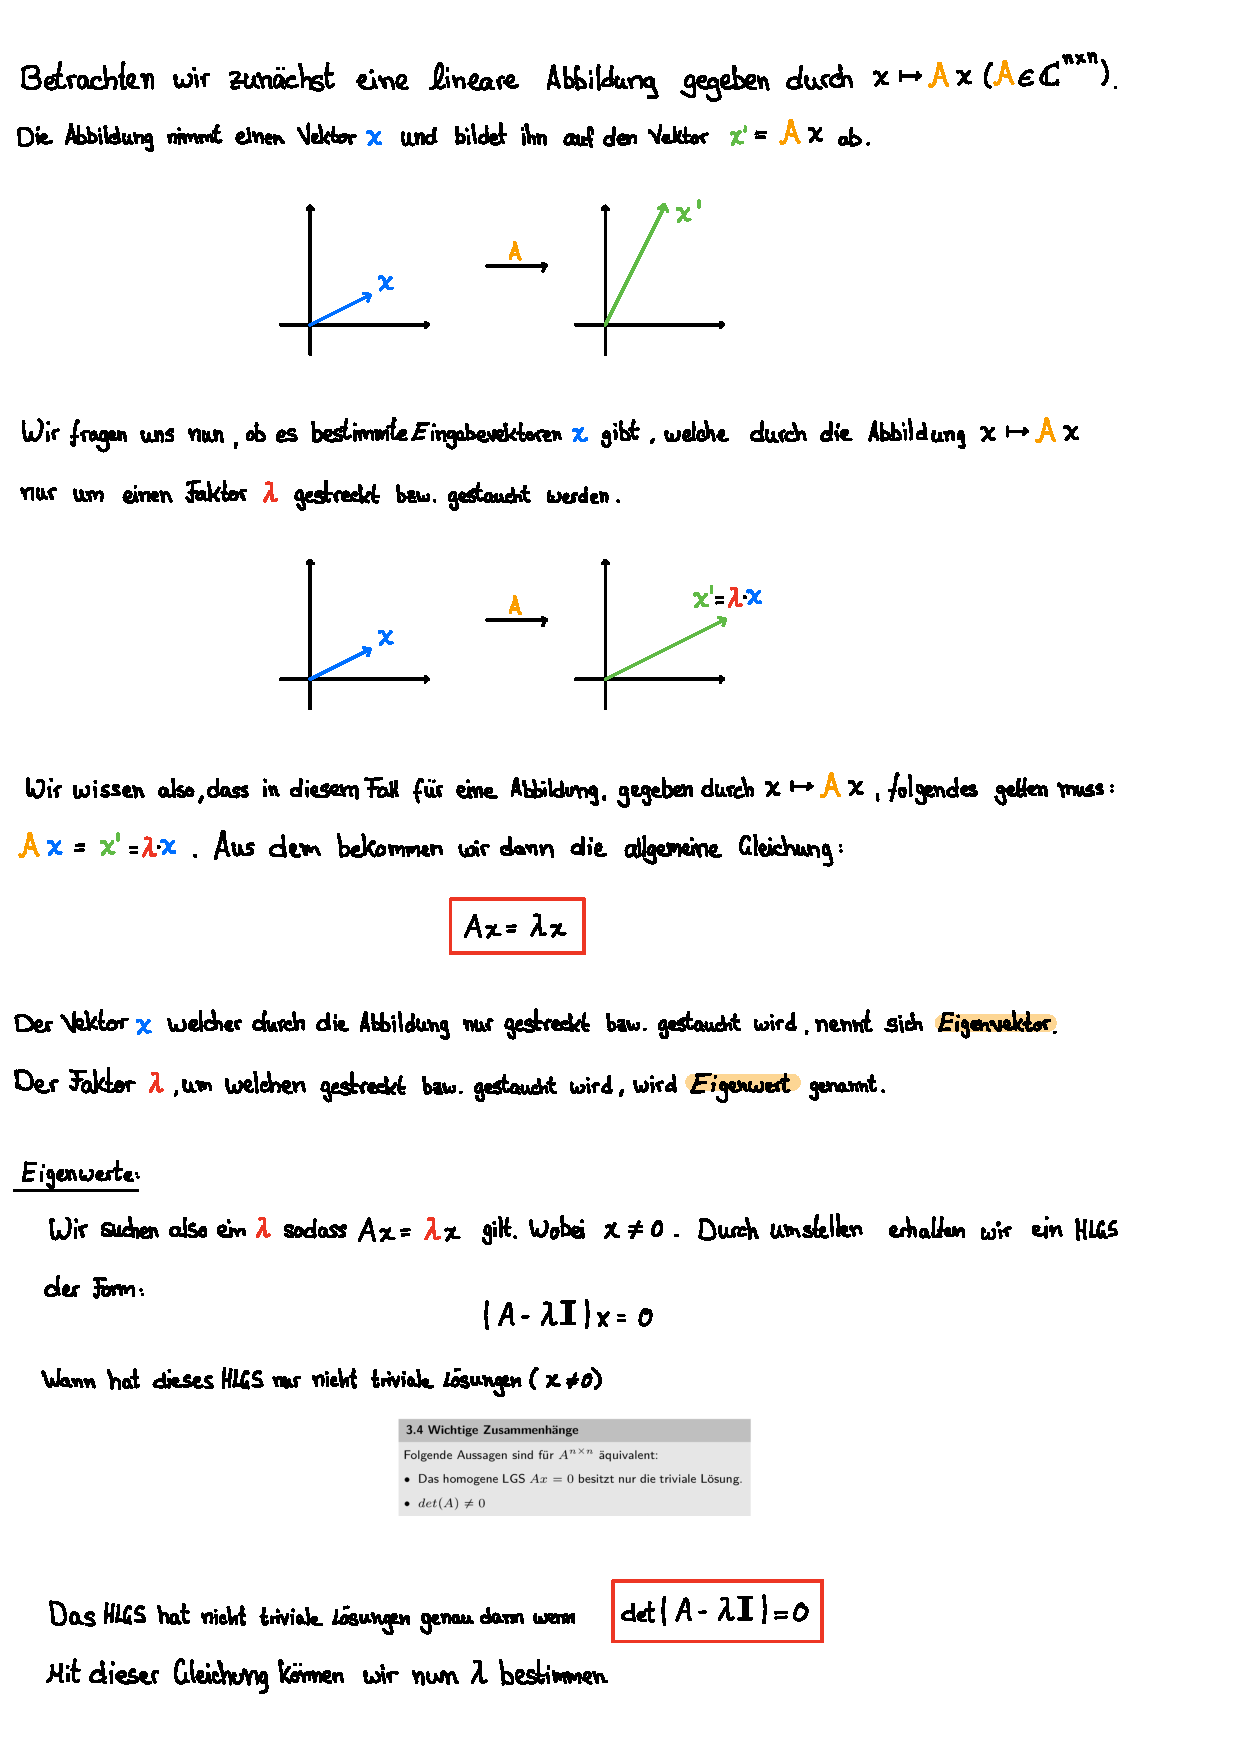
\includegraphics[page=1, scale=0.842]{pdf/06_Eigenwertproblem.pdf}
\end{figure}
\newpage
\includepdf[pages={2-}, 
            pagecommand={\thispagestyle{plain}}, 
            scale=0.95]{pdf/06_Eigenwertproblem.pdf}

\newgeometry{top=2.5cm, bottom=2cm}

\subsection{Beispielaufgaben} 

\vspace{1cm}

\subsubsection{} %Zardini S.93

Sei 

\begin{equation*}
    A = \begin{pmatrix}
    -3 & 4 & -4 \\
    0 & 5 & -8 \\
    0 & 4 & -7 \\
    \end{pmatrix}.
\end{equation*}

Bestimmen Sie die Eigenwerte und Eigenvektoren von \( A \) und geben Sie die geometrischen und algebraischen Vielfachheiten an. \\

\vspace{1\baselineskip}

\begin{solution}    

    \vspace{1\baselineskip}

    \leftskip=2em

    Eigenwerte durch det\( (A - \lambda \mathbb{I}) = 0 \) bestimmen. 

    \begin{equation*}
        \begin{aligned}
            \rightarrow & \begin{vmatrix}
                -3 - \lambda & 4 & -4 \\
                0 & 5 - \lambda & -8 \\
                0 & 4 & -7 - \lambda \\
            \end{vmatrix} = (-3 - \lambda) \begin{vmatrix}
                5 - \lambda & -8 \\
                4 & -7 - \lambda \\
                \end{vmatrix} \\[0.5em]
                &= \underbrace{(-3 - \lambda)}_{\lambda_1 = -3} \left[(5 - \lambda)(-7 - \lambda) + 32\right] = 0 \\[0.5em]
                \rightarrow & (5 - \lambda)(-7 - \lambda) + 32 = \lambda^2 + 2\lambda - 3 = \underbrace{(\lambda +3)}_{\lambda_2 = -3}\underbrace{(\lambda -1)}_{\lambda_3 = 1} = 0 
        \end{aligned}
    \end{equation*}

    Die Eigenwerte sind also \( \underbrace{\lambda_{1,2} = -3}_{\text{alg. vfh. 2}} \), und \( \underbrace{\lambda_3 = 1}_{\text{alg. vfh. 1}} \).

    \vspace{1\baselineskip}

    Nun die Eigenvektoren 

    \vspace{0.5\baselineskip}

    \( \rightarrow E_{-3}: \)
    \begin{equation*}
        \begin{gmatrix}[L]
            0 & 4 & -4 \\
            0 & 8 & -8 \\
            0 & 4 & -4 
        \end{gmatrix} \hspace{-0.75em} \begin{gmatrix}[R]
            0 \\ 0 \\ 0
        \end{gmatrix} \; \rightarrow \; \begin{gmatrix}[L]
            0 & 1 & -1 \\
            0 & 0 & 0 \\
            0 & 0 & 0
        \end{gmatrix} \hspace{-0.75em} \begin{gmatrix}[R]
            0 \\ 0 \\ 0
        \end{gmatrix} \; \rightarrow \; \begin{aligned}
            x_3 &= t \\
            x_2 &= s \\
            x_1 &= s
        \end{aligned} \qquad E_{-3} = \text{span} \left\{ \begin{pmatrix}
            1 \\ 0 \\ 0
        \end{pmatrix}, \begin{pmatrix}
            0 \\ 1 \\ 1
        \end{pmatrix} \right\} 
    \end{equation*}

    Die geometrische Vielfachheit von \( \lambda_{1,2} \) ist 2. 

    \vspace{1\baselineskip}

    \( \rightarrow E_{1}: \)
    \begin{equation*}
        \begin{gmatrix}[L]
            -4 & 4 & -4 \\
            0 & 4 & -8 \\
            0 & 4 & -8 
        \end{gmatrix} \hspace{-0.75em} \begin{gmatrix}[R]
            0 \\ 0 \\ 0
        \end{gmatrix} \; \rightarrow \; \begin{gmatrix}[L]
            -1 & 1 & -1 \\
            0 & 1 & -2 \\
            0 & 0 & 0 
        \end{gmatrix} \hspace{-0.75em} \begin{gmatrix}[R]
            0 \\ 0 \\ 0
        \end{gmatrix} \; \rightarrow \; \begin{aligned}
            x_3 &= t \\
            x_2 &= 2t \\
            x_1 &= 2t - t
        \end{aligned} \qquad E_{1} = \text{span} \left\{ \begin{pmatrix}
            1 \\ 2 \\ 1
        \end{pmatrix} \right\}
    \end{equation*}

    Die geometrische Vielfachheit von \( \lambda_{3} \) ist 1.

\end{solution}

\newpage

\subsubsection{} %Zardini S.96

Sei 

\begin{equation*}
    A = \begin{pmatrix}
    -3 & 4 & -4 \\
    0 & 5 & -8 \\
    0 & 4 & -7 \\
    \end{pmatrix}.
\end{equation*}

\begin{enumerate}[label=\alph*)]
    \item Berechnen Sie das charakteristische Polynom von \( A \) und überprüfen Sie ob \( A \) diagonalisierbar ist.
    \item Falls möglich, diagonalisieren Sie \( A \), sodass \[ D = T^{-1}AT\]
    \item Kann \( T \) orthogonal gewählt werden? Falls ja, geben Sie ein solches \( T \) an.
\end{enumerate}

\vspace{1\baselineskip}

\begin{solution}    

    \vspace{1\baselineskip}

    \leftskip=2em

    \textbf{a)} Aus 6.6.1 kennen wir bereits das charakteristische Polynom \[ p_A(\lambda) = (-3 - \lambda) \left[ (5 - \lambda)(-7 - \lambda) + 32 \right] = - (\lambda + 3)^2(\lambda - 1). \] Wir sahen auch, dass für jeden Eigenwert geom. Vfh. = alg. Vfh. gilt. Die Matrix ist also halbeinfach und deswegen Diagonalisierbar.

    \vspace{1\baselineskip}

    \textbf{b)} Mit den Eigenwerten und Eigenvektoren aus 6.6.1 können wir auch schnell \( D \) unf \( T \) aufschreiben. 

    \begin{equation*}
        D = \begin{pmatrix}
        -3 & 0 & 0 \\
        0 & -3 & 0 \\
        0 & 0 & 1 
        \end{pmatrix} \quad \text{und} \quad T = \begin{pmatrix}
            1 & 0 & 1 \\
            0 & 1 & 2 \\
            0 & 1 & 1 \\
        \end{pmatrix}
    \end{equation*}

    \vspace{1\baselineskip}

    \textbf{c)} \( T \) kann nicht orthogonal gewählt werden, da \( A \) nicht symmetrisch ist.

\end{solution}

\newpage

\subsubsection{} %Zardini S. 107

Sei \[ A = \begin{pmatrix} 5 & -6 \\ 3 & -4 \\ \end{pmatrix}. \] Berechnen Sie \( e^A \).

\vspace{1\baselineskip}

\textit{Tipp}: Das Matrixexponential vereinfacht sich für diagonalisierbare Matrizen als 
\[e^A = \sum_{n=0}^{\infty} \frac{A^n}{n!} = Tdiag(e^{\lambda_1}, ..., e^{\lambda_n})T^{-1}.\]

\vspace{1\baselineskip}

\begin{solution}    

    \vspace{1\baselineskip}

    \leftskip=2em

    Wir diagonalisieren \( A \) und berechnen dann \( e^A \) mit der Formel aus der Aufgabenstellung.

    \vspace{1\baselineskip}

    Eigenwerte:

    \begin{equation*}
        \begin{vmatrix}
            5 - \lambda & -6 \\
            3 & -4 - \lambda \\
        \end{vmatrix} = (5 - \lambda)(-4 - \lambda) + 18 = \lambda^2 - \lambda - 2 = (\lambda - 2)(\lambda + 1) = 0
    \end{equation*}

    \begin{equation*}
        \lambda_1 = -1, \quad \lambda_2 = 2
    \end{equation*}

    Eigenvektoren:

    \vspace{0.5\baselineskip}

    \( \rightarrow E_{-1} \):
    \begin{equation*}
        \begin{gmatrix}[L]
            6 & -6 \\
            3 & -3 
        \end{gmatrix} \hspace{-0.75em} \begin{gmatrix}[R]
            0 \\ 0
        \end{gmatrix} \; \rightarrow \; \begin{gmatrix}[L]
            1 & -1 \\
            0 & 0 
        \end{gmatrix} \hspace{-0.75em} \begin{gmatrix}[R]
            0 \\ 0
        \end{gmatrix} \; \rightarrow \; \begin{aligned}
            x_2 &= t \\
            x_1 &= t
        \end{aligned}  
        \qquad E_{-1} = \text{span} \left\{ \begin{pmatrix}
            1 \\ 1
        \end{pmatrix} \right\}
    \end{equation*}

    \( \rightarrow E_{2} \):
    \begin{equation*}
        \begin{gmatrix}[L]
            3 & -6 \\
            3 & -6 
        \end{gmatrix} \hspace{-0.75em} \begin{gmatrix}[R]
            0 \\ 0
        \end{gmatrix} \; \rightarrow \; \begin{gmatrix}[L]
            1 & -2 \\
            0 & 0 
        \end{gmatrix} \hspace{-0.75em} \begin{gmatrix}[R]
            0 \\ 0
        \end{gmatrix} \; \rightarrow \; \begin{aligned}
            x_2 &= t \\
            x_1 &= 2t
        \end{aligned}  
        \qquad E_{2} = \text{span} \left\{ \begin{pmatrix}
            2 \\ 1
        \end{pmatrix} \right\}
    \end{equation*}

    \begin{equation*}
        T = \begin{pmatrix}
            1 & 2 \\
            1 & 1
        \end{pmatrix}, \quad T^{-1} = \begin{pmatrix}
            -1 & 2 \\
            1 & -1
        \end{pmatrix}
    \end{equation*}

    Das Matrixexponential ist also

    \begin{equation*}
        e^A = \begin{pmatrix}
            1 & 2 \\
            1 & 1
        \end{pmatrix} \begin{pmatrix}
            e^{-1} & 0 \\
            0 & e^{2}
        \end{pmatrix} \begin{pmatrix}
            -1 & 2 \\
            1 & -1
        \end{pmatrix} = \begin{pmatrix}
            -e^{-1} + 2e^{2} & 2e^{-1} - 2e^{2} \\
            -e^{-1} + e^{2} & 2e^{-1} - e^{2}
        \end{pmatrix}
    \end{equation*}

\end{solution}

\newpage

\subsubsection{} %Zardini S. 110

Sei die quadratische Form \( q \) gegeben durch \[ \begin{aligned} q: \; \mathbb{R}^2 &\rightarrow \mathbb{R} \\ q(x) &\mapsto \frac{1}{2}x_1^2 + \sqrt{3}x_1x_2-\frac{1}{2}x_2^2 \;, \;x= \begin{pmatrix} x_1 \\ x_2\\ \end{pmatrix} \end{aligned} \]

\begin{enumerate}[label=\alph*)]
    \item Bestimmen Sie eine symmetrische Matrix \( A \), sodass \( q(x)=x^\top Ax \).
    \item Führen Sie die Hauptachsentransformation \( y=Tx \) durch und geben Sie die Normalform von \( q \) an.
\end{enumerate}

\vspace{1\baselineskip}

\begin{solution}    

    \vspace{1\baselineskip}

    \leftskip=2em

    \textbf{a)} \( A = \begin{pmatrix} \frac{1}{2} & \frac{\sqrt{3}}{2} \\ \frac{\sqrt{3}}{2} & -\frac{1}{2} \end{pmatrix} \)

    \vspace{1\baselineskip}

    \textbf{b)} Diagonalisieren:

    \begin{equation*}
        \begin{vmatrix}
            \frac{1}{2} - \lambda & \frac{\sqrt{3}}{2} \\
            \frac{\sqrt{3}}{2} & -\frac{1}{2} - \lambda
        \end{vmatrix} = \left(\frac{1}{2} - \lambda\right)\left(-\frac{1}{2} - \lambda\right) - \frac{3}{4} = \lambda^2 - 1 = 0 
    \end{equation*}

    \begin{equation*}
        \lambda_1 = -1, \quad \lambda_2 = 1
    \end{equation*}

    \begin{equation*}
        E_1: \begin{vmatrix}
            - \frac{1}{2} & \frac{\sqrt{3}}{2} \\
            \frac{\sqrt{3}}{2} & -\frac{3}{2}
        \end{vmatrix} \; \rightarrow \; E_1 = \text{span} \left\{ \begin{pmatrix}
            \sqrt{3} \\ 1
        \end{pmatrix} \right\}
    \end{equation*}

    \begin{equation*}
        E_{-1}: \begin{vmatrix}
            \frac{3}{2} & \frac{\sqrt{3}}{2} \\
            \frac{\sqrt{3}}{2} & \frac{1}{2}
        \end{vmatrix} \; \rightarrow \; E_{-1} = \text{span} \left\{ \begin{pmatrix}
            \frac{\sqrt{3}}{3} \\ -1
        \end{pmatrix} \right\}
    \end{equation*}

    Damit \( T \) orthogonal ist, müssen wir noch die Eigenvektoren normieren um dann \( T \) und \( D \) aufschreiben zu können. 

    \begin{equation*}
        T = \begin{pmatrix}
            \frac{\sqrt{3}}{2} & \frac{1}{2} \\
            \frac{1}{2} & -\frac{\sqrt{3}}{2} 
            \end{pmatrix}, \quad D = \begin{pmatrix}
                1 & 0 \\
                0 & -1
            \end{pmatrix}
    \end{equation*}

    Nun können wir die Hauptachsentransformation \( y = Tx \) durchführen.

    \begin{equation*}
        x^\top Ax \xrightarrow{x=T^{-1}y} (T^{-1}y)^\top A T^{-1}y = y^\top \underbrace{T A T^{-1}}_{D} y
    \end{equation*}

    \begin{equation*}
        \begin{pmatrix}
            y_1 & y_2
        \end{pmatrix} \begin{pmatrix}
            1 & 0 \\
            0 & -1
        \end{pmatrix} \begin{pmatrix}
            y_1 \\ y_2
        \end{pmatrix} = y_1^2 - y_2^2
    \end{equation*}

    \vspace{0.5\baselineskip}

    \begin{equation*}
        q(y) = y_1^2 - y_2^2
    \end{equation*}

\end{solution}